% begin module derivatives-as-function-ex2
\begin{frame}
\begin{example} %[Example 3, p. 148]
If $f(x) = x^3-x$, find the formula for $f'(x)$.
\begin{columns}[c]
\column{.25\textwidth}
\psset{xunit=0.7cm, yunit=0.7cm}
\begin{pspicture}(-2,-2.5)(2,2.5)
\psframe*[linecolor=white](-2,-2.5)(2,2.5)
\psaxes[ticks=none, labels=none]{<->}(0,0)(-2,-2.5)(2,2.5)
%Function formula: - (x)+(x)^{3} 
\psplot[linecolor=red, plotpoints=1000]{-1.5}{1.5}{x 3 exp x -1 mul add }
\tiny
\psLabelXOne
\psLabelYOne
\rput[l](-1.3, 0.6){$y=f(x)$}
\end{pspicture} 
%\ 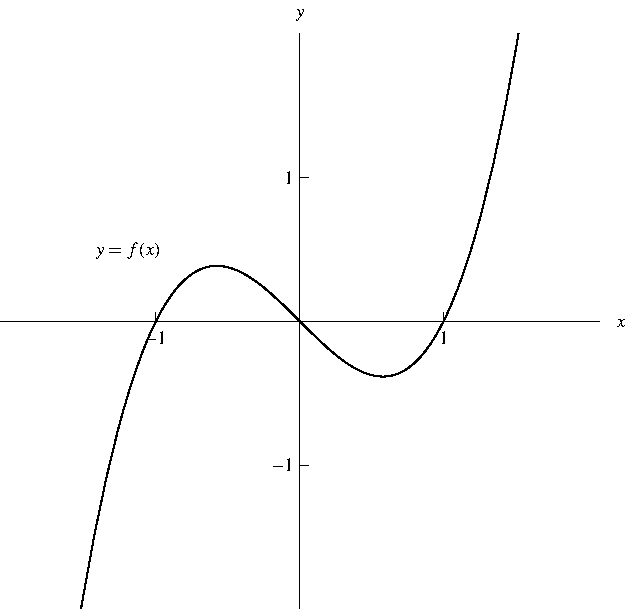
\includegraphics[height=3cm]{derivatives/pictures/03-02-ex2a.pdf}%
%\ \only<handout:0| -7>{%
%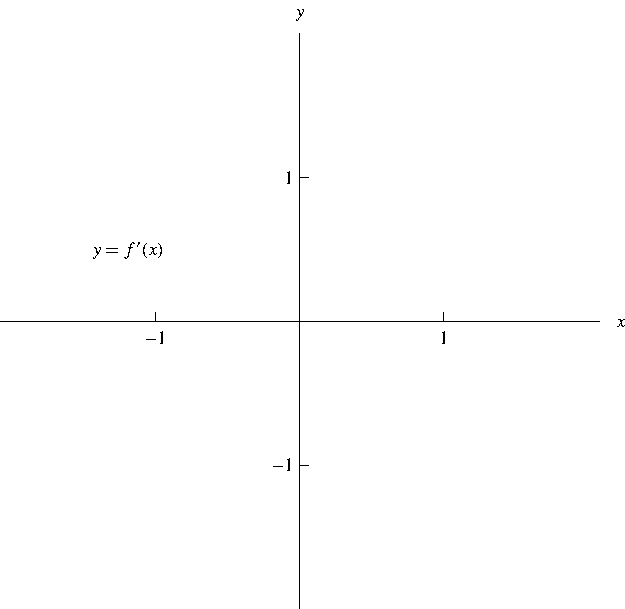
\includegraphics[height=3cm]{derivatives/pictures/03-02-ex2b.pdf}%
%}%
%\only<8->{%
%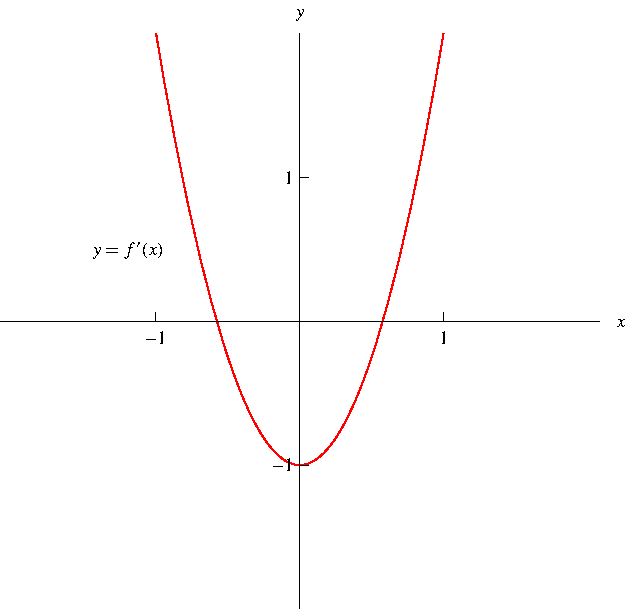
\includegraphics[height=3cm]{derivatives/pictures/03-02-ex2c.pdf}%
%}%

\psset{xunit=0.7cm, yunit=0.7cm}
\begin{pspicture}(-2,-2.5)(2,2.5)
\psframe*[linecolor=white](-2,-2.5)(2,2.5)
\psaxes[ticks=none, labels=none]{<->}(0,0)(-2,-2.5)(2,2.5)
\tiny
\psLabelXOne
\psLabelYOne
%Function formula: 3 ((x)^{2})-1 
\uncover<8->{
\psplot[linecolor=blue, plotpoints=1000]{-1}{1}{-1 x 2 exp 3 mul add }
\rput[l](-1.3, -1.5){$y=f(x)$}
}
\end{pspicture} 
\column{.75\textwidth}
\begin{align*}
&\uncover<2->{f'(x)}\\%
 & \uncover<2->{ = } %
\uncover<2->{\lim_{h\rightarrow 0} \frac{f(x+h)-f(x)}{h}}\\%
 & \uncover<3->{ = } %
\uncover<3->{\lim_{h\rightarrow 0} \frac{[(x+h)^3 - (x+h)]-[x^3-x]}{h}}\\%
 & \uncover<4->{ = } %
\uncover<4->{\lim_{h\rightarrow 0} \frac{x^3 + 3x^2h+3xh^2+h^3-x-h-x^3+x}{h}}\\%
 & \uncover<5->{ = } %
\uncover<5->{\lim_{h\rightarrow 0} \frac{3x^2h+3xh^2+h^3-h}{h}}\\%
 & \uncover<6->{ = } %
\uncover<6->{\lim_{h\rightarrow 0} (3x^2+3xh+h^2-1)}\\%
 & \uncover<7->{ = } %
\uncover<7,8->{3x^2-1}%
\end{align*}
\end{columns}
\end{example}
\end{frame}
% end module derivatives-as-function-ex2
